\documentclass[10pt]{beamer}
\usepackage{listings}
\usetheme{uha}
\usepackage{hyperref}
\usepackage{indentfirst}
\usepackage{booktabs}
\usepackage{multirow}
\usepackage{xeCJK}
\usepackage[french,english]{babel}
\usepackage[T1]{fontenc}
\usepackage[utf8]{inputenc}
\usepackage{amsmath}
\usepackage{amsfonts}
\usepackage{amssymb}
%\usepackage{tikz}
\setmainfont{Ubuntu}
\title{代码编程相关工作介绍}
\subtitle{Coding Job Introduce}
\date{\today}
\author{haobo.gao}
\institute{ZhengZhou}

\lstset{
	numbers=left,
	numberstyle=\tiny,
	basicstyle=\scriptsize,
	backgroundcolor= \color{gray},
	keywordstyle=\color{blue!70},
	breaklines=true,
	breakautoindent=true,
	breakindent=4em,
	commentstyle=\color{codegreen},
	frame=shadowbox,
	escapeinside=``,
	tabsize=4,
	framextopmargin=1pt,framexbottommargin=1pt,abovecaptionskip=-1pt,belowcaptionskip=1pt,
  xleftmargin=3em,xrightmargin=3em,
	language=C
}


\begin{document}




% Title page 标题页
\begin{frame}[plain, noframenumbering]
	\titlepage
\end{frame}



%=============================================================================================
\section{Introduction}

%------------------------------------------------
\begin{frame}[fragile]{职位}

	和代码相关的职位方向主要有:
	\begin{itemize}
		\item 脚本开发方向
		\item 前端开发方向
		\item 应用开发方向
		\item 系统级开发方向
		\item 底层开发方向
	\end{itemize}
\end{frame}

%--------------------------------------------
\begin{frame}[fragile]{工作执掌介绍}

		为了更清晰的表达,首先总体介绍一下一台计算机包含的所有和代码
	有关的技术  。 目的是让你对计算机科学有初步的认识。接下来会有
	一张计算机的硬件构成框图。帮助你认知。


\end{frame}

%--------------------------------------------
\begin{frame}[fragile]{计算机硬件介绍}

	下图是计算机的原理图,我们的电脑无非就有如下的核心模块:
	\begin{figure}[htbp]
	\begin{center}
	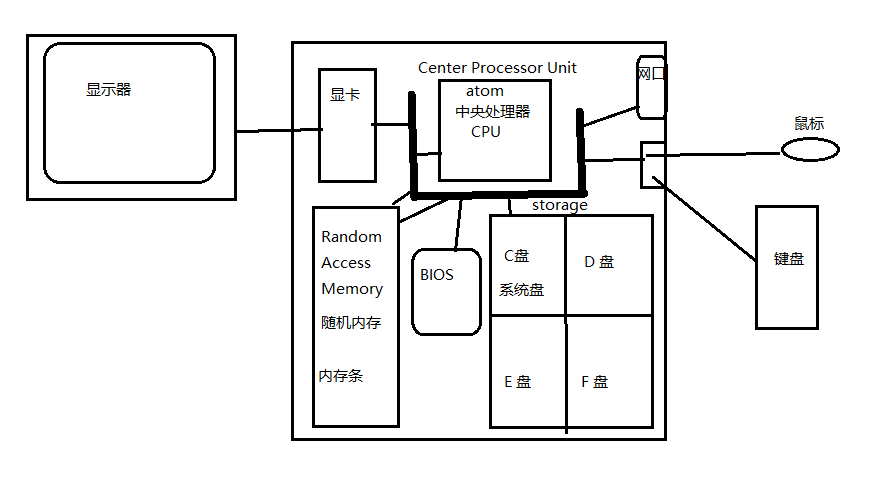
\includegraphics[width=10cm]{img/cmptfrom}
	\caption{计算机组成}
	\label{cmptfrom}
	\end{center}
	\vspace{-0.5em}
	\end{figure}
	\end{frame}

%--------------------------------------------
\begin{frame}[fragile]{CPU:机器码 }

CPU 全称是 Center Processor Unit .主要执行算术计算。CPU 被发明出来后,会有一套厂商规定的基础指令。
如 intel 的 cpu 使用的是 X86 指令集。 指令是二进制的数字(又叫做机器码),这些二进制数字可以直接被CPU 识别,
从而用于命令CPU 做事情。
\end{frame}
%--------------------------------------------
\begin{frame}[fragile]{CPU:机器码时代 }
前面已经告诉你,计算机的CPU 主要是识别用户的机器码来进行运算。但是机器码是规定的二进制的数字,我们需要CPU
帮我们计算 1+1 等于几的时候对应的机器码 是 :
\begin{verbatim}
00010000 r0 00000001 00000001
\end{verbatim}
\end{frame}

%--------------------------------------------
\begin{frame}[fragile]{CPU:汇编 }
随着计算机的发展,机器码的效率十分低。 此时人们设计了汇编语言。汇编是一个解释翻译器,当你
输入add ,1 ,1,r0的时候,这个编译器会自动把你的代码转换为机器码。 而这个过程就叫做编译。
汇编语言书写 1 + 1 的代码是:
\begin{lstlisting}
add 1 1 r0
\end{lstlisting}

\end{frame}


%--------------------------------------------
\begin{frame}[fragile]{RAM and Storage }

好了,现在你知道 CPU 可以读取指令来执行,产生结果。
那么从哪里获取指令呢?

答案是 memory .  计算机的memory 指的是拥有地址空间的
记忆单元。
\end{frame}

%--------------------------------------------
\begin{frame}[fragile]{memory}

memory 的逻辑样子就是这样的:
\begin{figure}[htbp]
\begin{center}
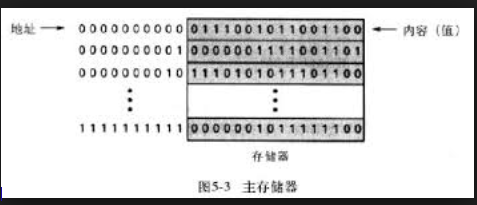
\includegraphics[width=6cm]{img/memory}
\caption{memory 逻辑图}
\label{memory}
\end{center}
\vspace{-0.5em}
\end{figure}

\end{frame}


%--------------------------------------------
\begin{frame}[fragile]{RAM and Storage }

RAM 就是内存,是一种memory ,我们常说的内存条就是这个东西。它有如下特性:
\begin{itemize}
\item 速度快。CPU 可以直接寻址。
\item 掉电数据丢失,成本高,容量小。
\end{itemize}

Storage 是 存储。 我们通常用的 磁盘,储存卡等 都归类为储存。它有如下特性:
\begin{itemize}
\item 速度慢。CPU 无法直接寻址。
\item 掉电数据不丢失,成本较低,容量大。
\end{itemize}

\end{frame}



%--------------------------------------------
\begin{frame}[fragile]{代码的执行}
写好的代码会在storage 中,被CPU 加载到 内存中,然后执行。

CPU 上电的第一条指令是再BIOS中执行。BIOS 加载 磁盘中C盘的操作系统代码到内存中。然后CPU 执行
操作系统代码。

接下来操作系统执行,加载各个系统模块,这样就有了我们电脑刚开机的样子。


\end{frame}



%========================================================================================================
\section{计算机软件架构}

%-----------------------------------------------
\begin{frame}[fragile]{要介绍的术语}

这里主要介绍 以下一些 概念
\begin{itemize}
\item bootloader 启动代码
\item 操作系统
\item 操作系统驱动
\item 操作系统应用
\item UI 和其他逻辑
\end{itemize}

\end{frame}


%-----------------------------------------------
\begin{frame}{Les listes}
	item
	\begin{itemize}
		\item Premier
		\item Second
		\item Troisième
	\end{itemize}

	枚举
	\begin{enumerate}
		\item Premier
		\item Second
		\item Troisième
	\end{enumerate}

	描述
	\begin{description}
		\item [UHA] Université de Haute Alsace
	\end{description}
\end{frame}

%-----------------------------------------------
\begin{frame}{Les blocks}
	\begin{exampleblock}{示例一}
		示例
	\end{exampleblock}
	\begin{alertblock}{提醒}
		提醒
	\end{alertblock}
	\begin{block}{普通}
		普通
	\end{block}
\end{frame}



\end{document}
